\documentclass[10pt,leter,openany]{article}
\usepackage[latin1]{inputenc}
\usepackage[english]{babel}
\usepackage{amsmath}
\usepackage{amsfonts}
\usepackage{amssymb}
\usepackage{graphicx}
\usepackage{listings}
\usepackage{color}
\usepackage[left=3cm,right=3cm,top=3cm,bottom=3cm]{geometry}
\usepackage[numbers,sort&compress]{natbib}
\usepackage{url}
\usepackage{caption}
\usepackage{siunitx}
%\usepackage{subfigure}
\usepackage{float}
\usepackage{booktabs}
\usepackage{subcaption}
\usepackage{comment}
\usepackage{mwe}
%\usepackage[table,xcdraw]{xcolor}
\usepackage[shortlabels]{enumitem}   %To enumerate with letters
\usepackage{mathtools}	%To write derivates
\usepackage[thinc]{esdiff}	%To write derivates
\usepackage{cancel} %To cancel terms in equations

\setlength{\parindent}{0pt}
\setlength{\parskip}{4pt}

\definecolor{mygreen}{rgb}{0,0.6,0}
\definecolor{mygray}{rgb}{0.5,0.5,0.5}
\definecolor{mymauve}{rgb}{0.58,0,0.82}

\lstset{ 
	backgroundcolor=\color{white},   % choose the background color; you must add \usepackage{color} or \usepackage{xcolor}; should come as last argument
	basicstyle=\footnotesize,        % the size of the fonts that are used for the code
	breakatwhitespace=false,         % sets if automatic breaks should only happen at whitespace
	breaklines=true,                 % sets automatic line breaking
	captionpos=b,                    % sets the caption-position to bottom
	commentstyle=\color{mygreen},    % comment style
	deletekeywords={...},            % if you want to delete keywords from the given language
	escapeinside={\%*}{*)},          % if you want to add LaTeX within your code
	extendedchars=true,              % lets you use non-ASCII characters; for 8-bits encodings only, does not work with UTF-8
	firstnumber=01,                	 % start line enumeration with line 1000
	frame=single,	                 % adds a frame around the code
	keepspaces=true,                 % keeps spaces in text, useful for keeping indentation of code (possibly needs columns=flexible)
	keywordstyle=\color{blue},       % keyword style
	language=Python,                 % the language of the code
	morekeywords={*,...},            % if you want to add more keywords to the set
	numbers=left,                    % where to put the line-numbers; possible values are (none, left, right)
	numbersep=5pt,                   % how far the line-numbers are from the code
	numberstyle=\tiny\color{mygray}, % the style that is used for the line-numbers
	rulecolor=\color{black},         % if not set, the frame-color may be changed on line-breaks within not-black text (e.g. comments (green here))
	showspaces=false,                % show spaces everywhere adding particular underscores; it overrides 'showstringspaces'
	showstringspaces=false,          % underline spaces within strings only
	showtabs=false,                  % show tabs within strings adding particular underscores
	stepnumber=1,                    % the step between two line-numbers. If it's 1, each line will be numbered
	stringstyle=\color{mymauve},     % string literal style
	tabsize=2,	                     % sets default tabsize to 2 spaces
	title=\lstname                   % show the filename of files included with \lstinputlisting; also try caption instead of title
}

\usepackage[dvipsnames,table,xcdraw]{xcolor}

\usepackage{fancyvrb}

% redefine \VerbatimInput
\RecustomVerbatimCommand{\VerbatimInput}{VerbatimInput}%
{fontsize=\footnotesize,
	%
	frame=lines,  % top and bottom rule only
	framesep=2em, % separation between frame and text
	rulecolor=\color{Gray},
	%
	label=\fbox{\color{Black}data.txt},
	labelposition=topline,
	%
	commandchars=\|\(\), % escape character and argument delimiters for
	% commands within the verbatim
	commentchar=*        % comment character
}



\usepackage{titling}
\newcommand{\subtitle}[1]{%
	\posttitle{%
		\par\end{center}
	\begin{center}\large#1\end{center}
	\vskip0.5em}%
}


\author{5273}
\title{Homework Assignment 10: Applied Probabilistic Models}
\subtitle{Monte Carlo Simulations}
\date{}


\begin{document}
	
\maketitle

\section{Introduction}
 In this work, Monte Carlo simulations are employed to estimate expected value in the exercises. To perform simulations, sampling distributions are considered to compare the expected values with the theoretical values obtained in the previous assignment.  
 
 The expected value of a random variable can be considered as the long-run average value of its outcomes when the number of repeated trials is large \citep{hanck2020}, and Monte Carlo simulations play an important role for this kind of experiments. An example of Monte Carlo simulation is repeating an experiment a large enough number of times to make the results practically equivalent to doing it over and over forever \citep{akbar2019}. 
 
 For the analysis, the R software is used in its version 4.0.2 \citep{r}, and the code used is available on the GitHub repository \citep{github}. This work is run on a MacBook Air with an Intel Core i5 CPU $ @ $ 1.8 GHz and 8 GB RAM.


\section{Exercises}

For this work exercises that have been simulated are provided in the book \citet{grinstead2012introduction}.

\subsection{Exercise 1 page 247}

For this exercise, a deck is given which consists of cards between 2 through 10. The player will win a dollar if the number of the card is odd and loses one dollar otherwise. The calculated expected value $E(X) = -\dfrac{1}{9}$. Then it is executed by simulations (10 000 repetitions), which yields very close values with respect to the previously calculated. In turn, other repetitions of this experiment are executed, represented in Figure \ref{fig:line}, which gives a threshold of all the expected values around the theoretical one.

\begin{figure}
	\begin{center}
		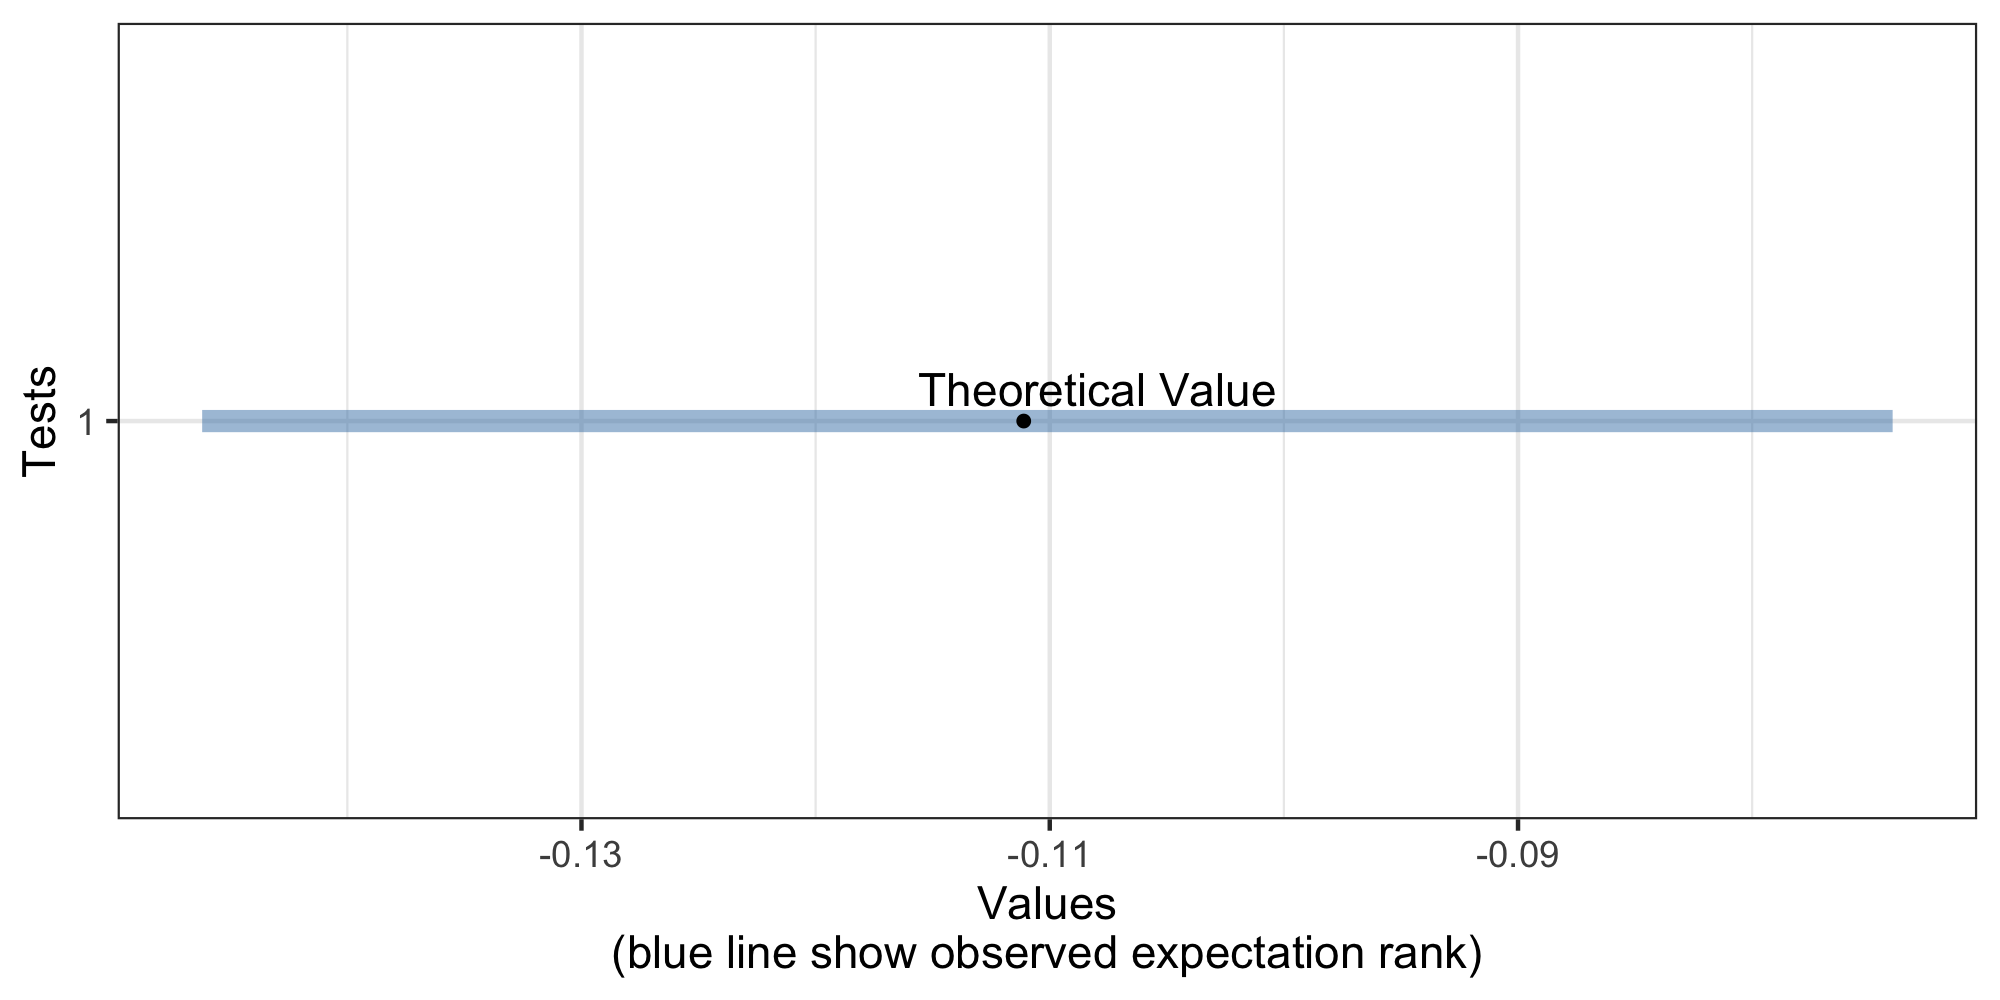
\includegraphics[scale=0.15]{img/line_1_247}
		\captionof{figure}{Expected value threshold in experiments in Exercise 1 page 247}
		\label{fig:line}
	\end{center}
\end{figure}

\subsection{Exercise 6 page 247}

In this situation, let $ X $ denote the sum of two numbers that turn up when a die is rolled twice, and $ Y $ the difference of the numbers. This exercise requires demonstrate that $ E(XY)=E(X)E(Y) $. As states before, simulations are executed to validate conclusions. The experiments are executed 10 000 times and then means are calculated the same amount of times also, Figure \ref{fig:box1} shows very similar results.

\begin{figure}
	\begin{center}
		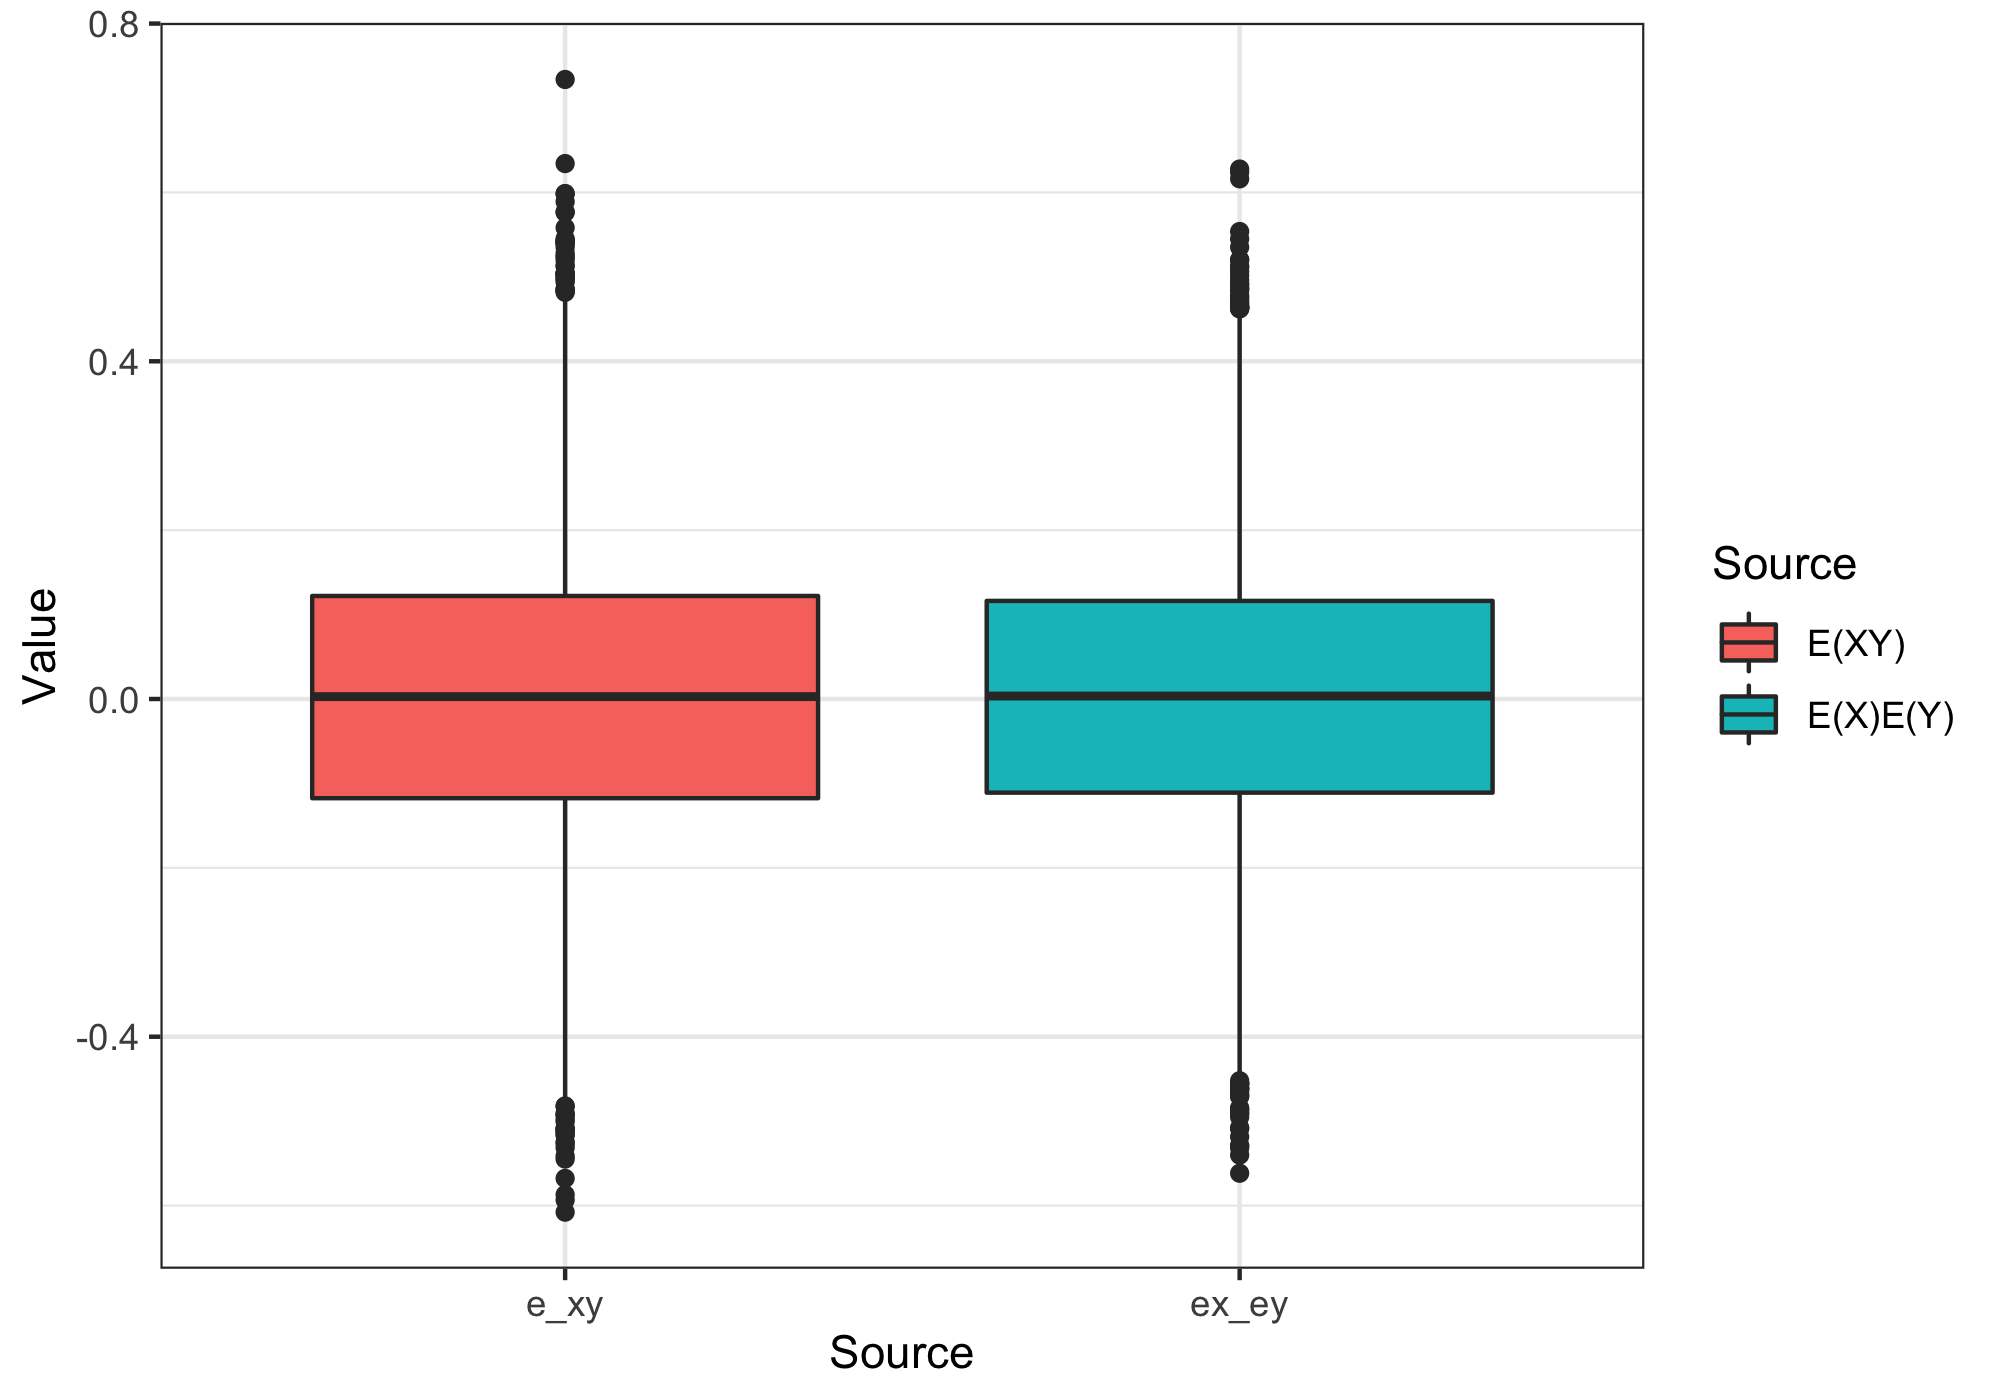
\includegraphics[scale=0.18]{img/boxplot1}
		\captionof{figure}{Boxplot of the expected values for both situations in Exercise 6 page 247}
		\label{fig:box1}
	\end{center}
\end{figure}
 
\subsection{Exercise 18 page 249}

In this exercise, six similar keys are given and let $ X $ be the number of tried keys before the success of opening the door. This situation gives an expected value $ E(X) = 2.5 $.  After computing, the sample means of 10 000 tries the experiment gives a value of 2.4818, which seems to be fairly close to the expected value. Figure \ref{fig:hist1} shows a histogram of the number of tries throughout the 10 000 repetitions of this Monte Carlo simulation. In addition, Figure \ref{fig:plotrepMC} represents a plot that shows after the value of 1 000 repetitions the expected value begins to stabilize, which is an approach to determine how many Monte Carlo experiments are enough.

\begin{figure}
	\begin{center}
		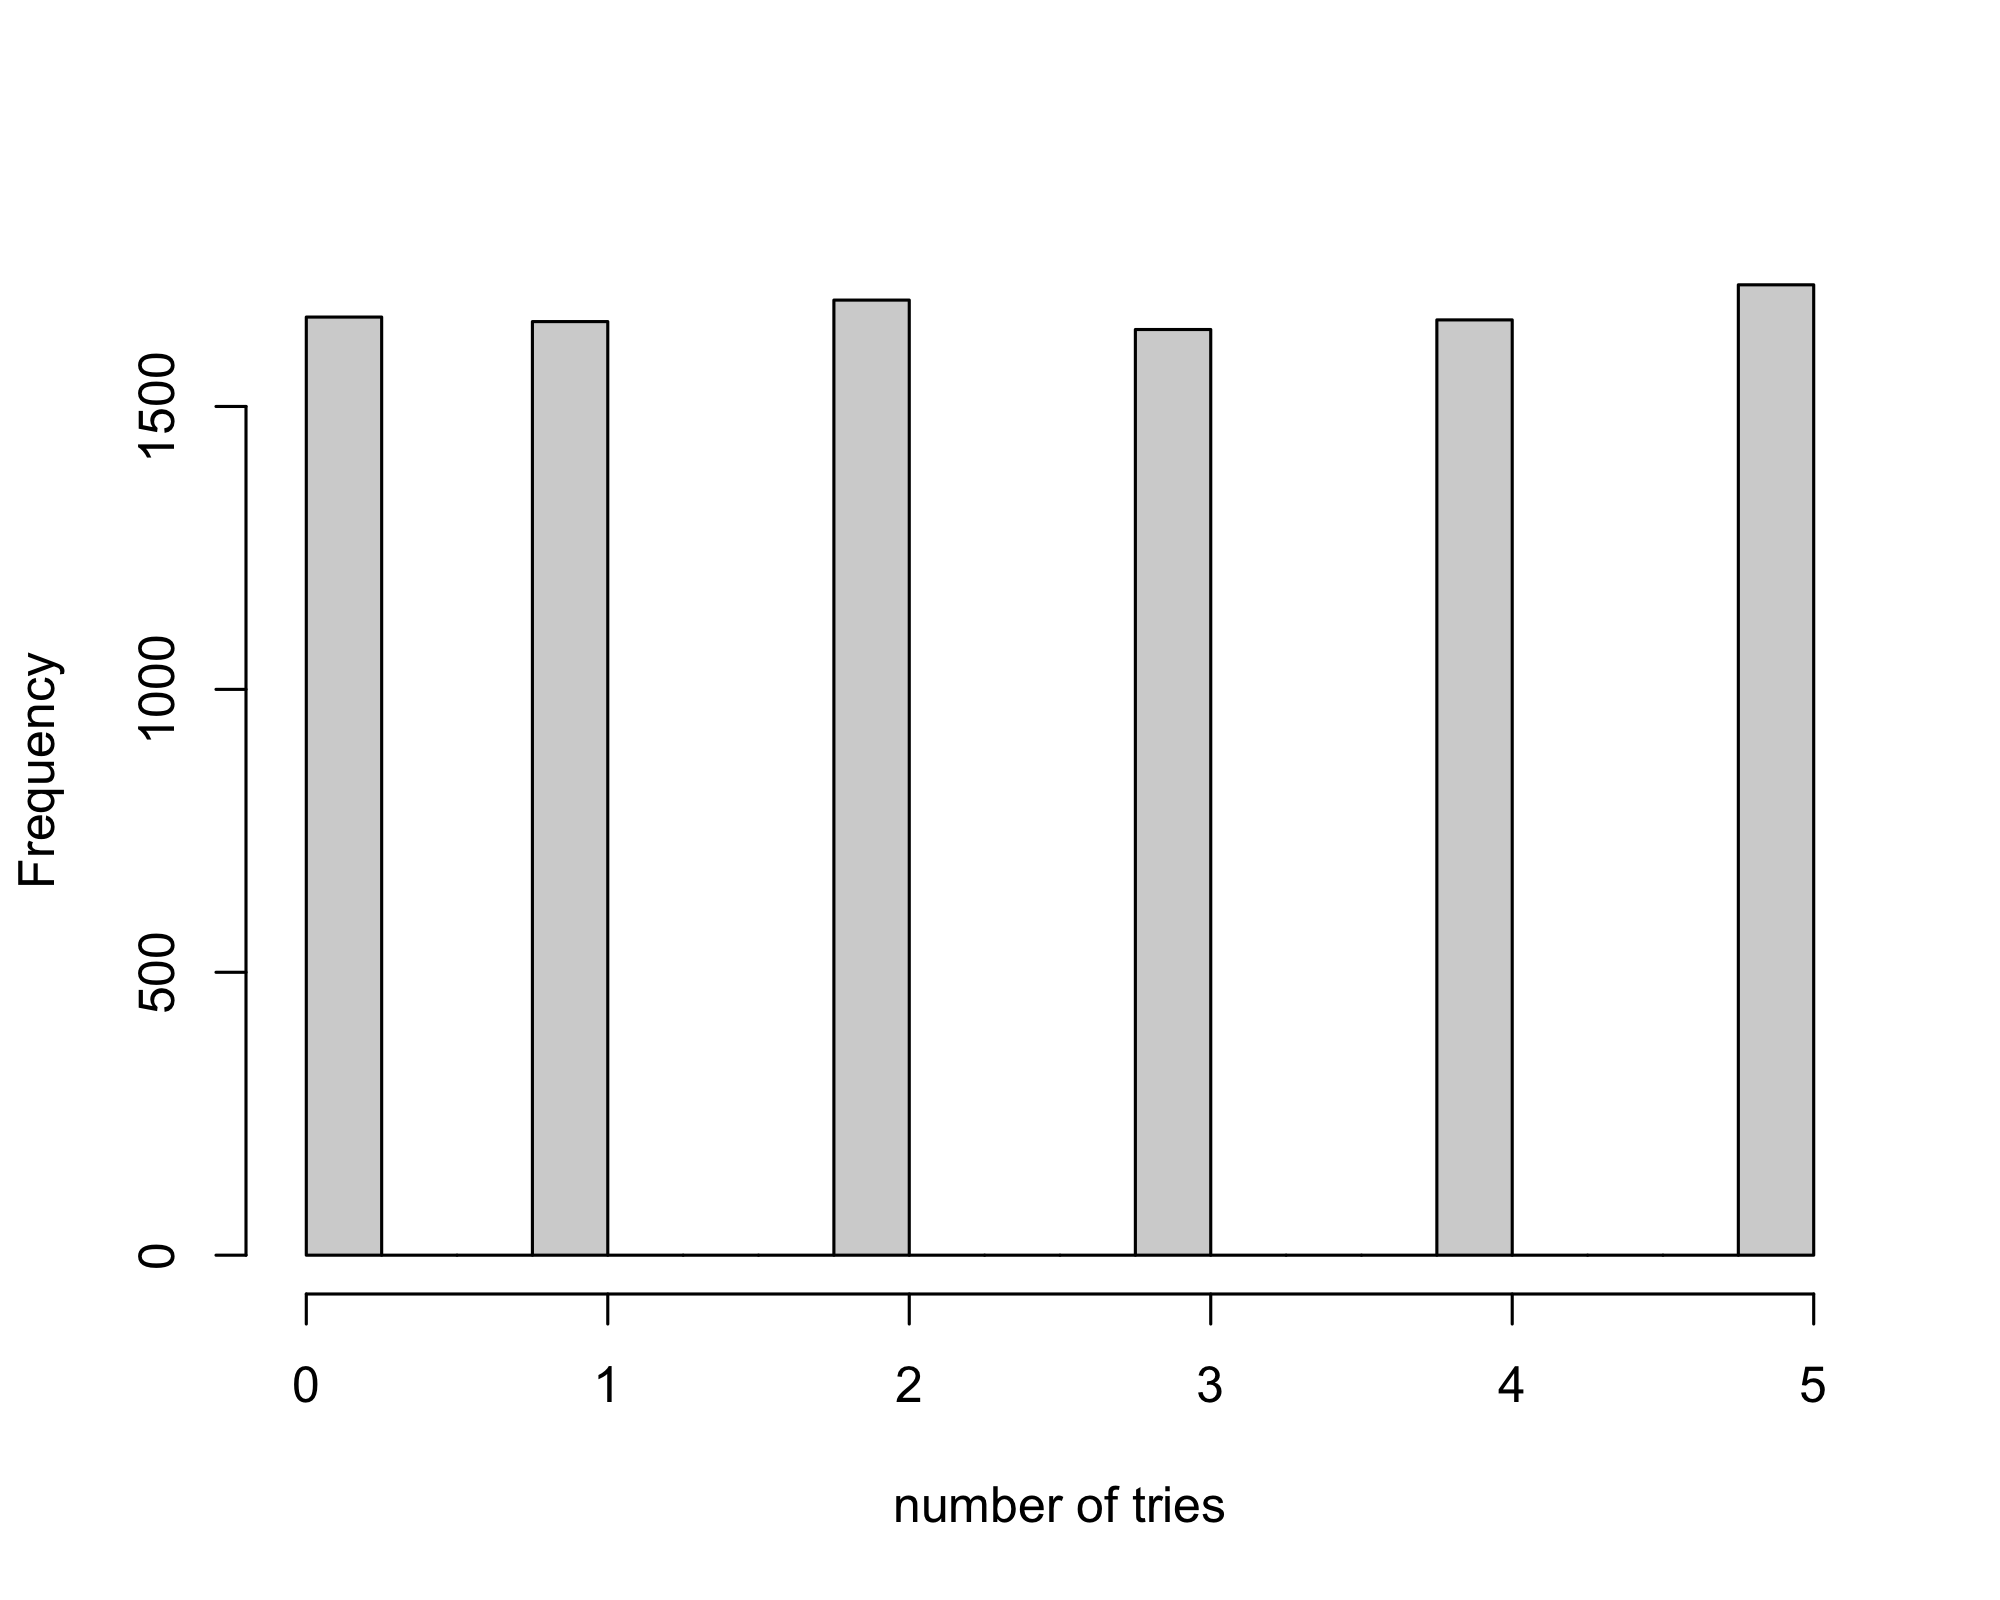
\includegraphics[scale=0.15]{img/hist_18_249}
		\captionof{figure}{Histogram of the number of tries before opening the door in Exercise 18 page 249}
		\label{fig:hist1}
	\end{center}
\end{figure}

\begin{figure}
	\begin{center}
		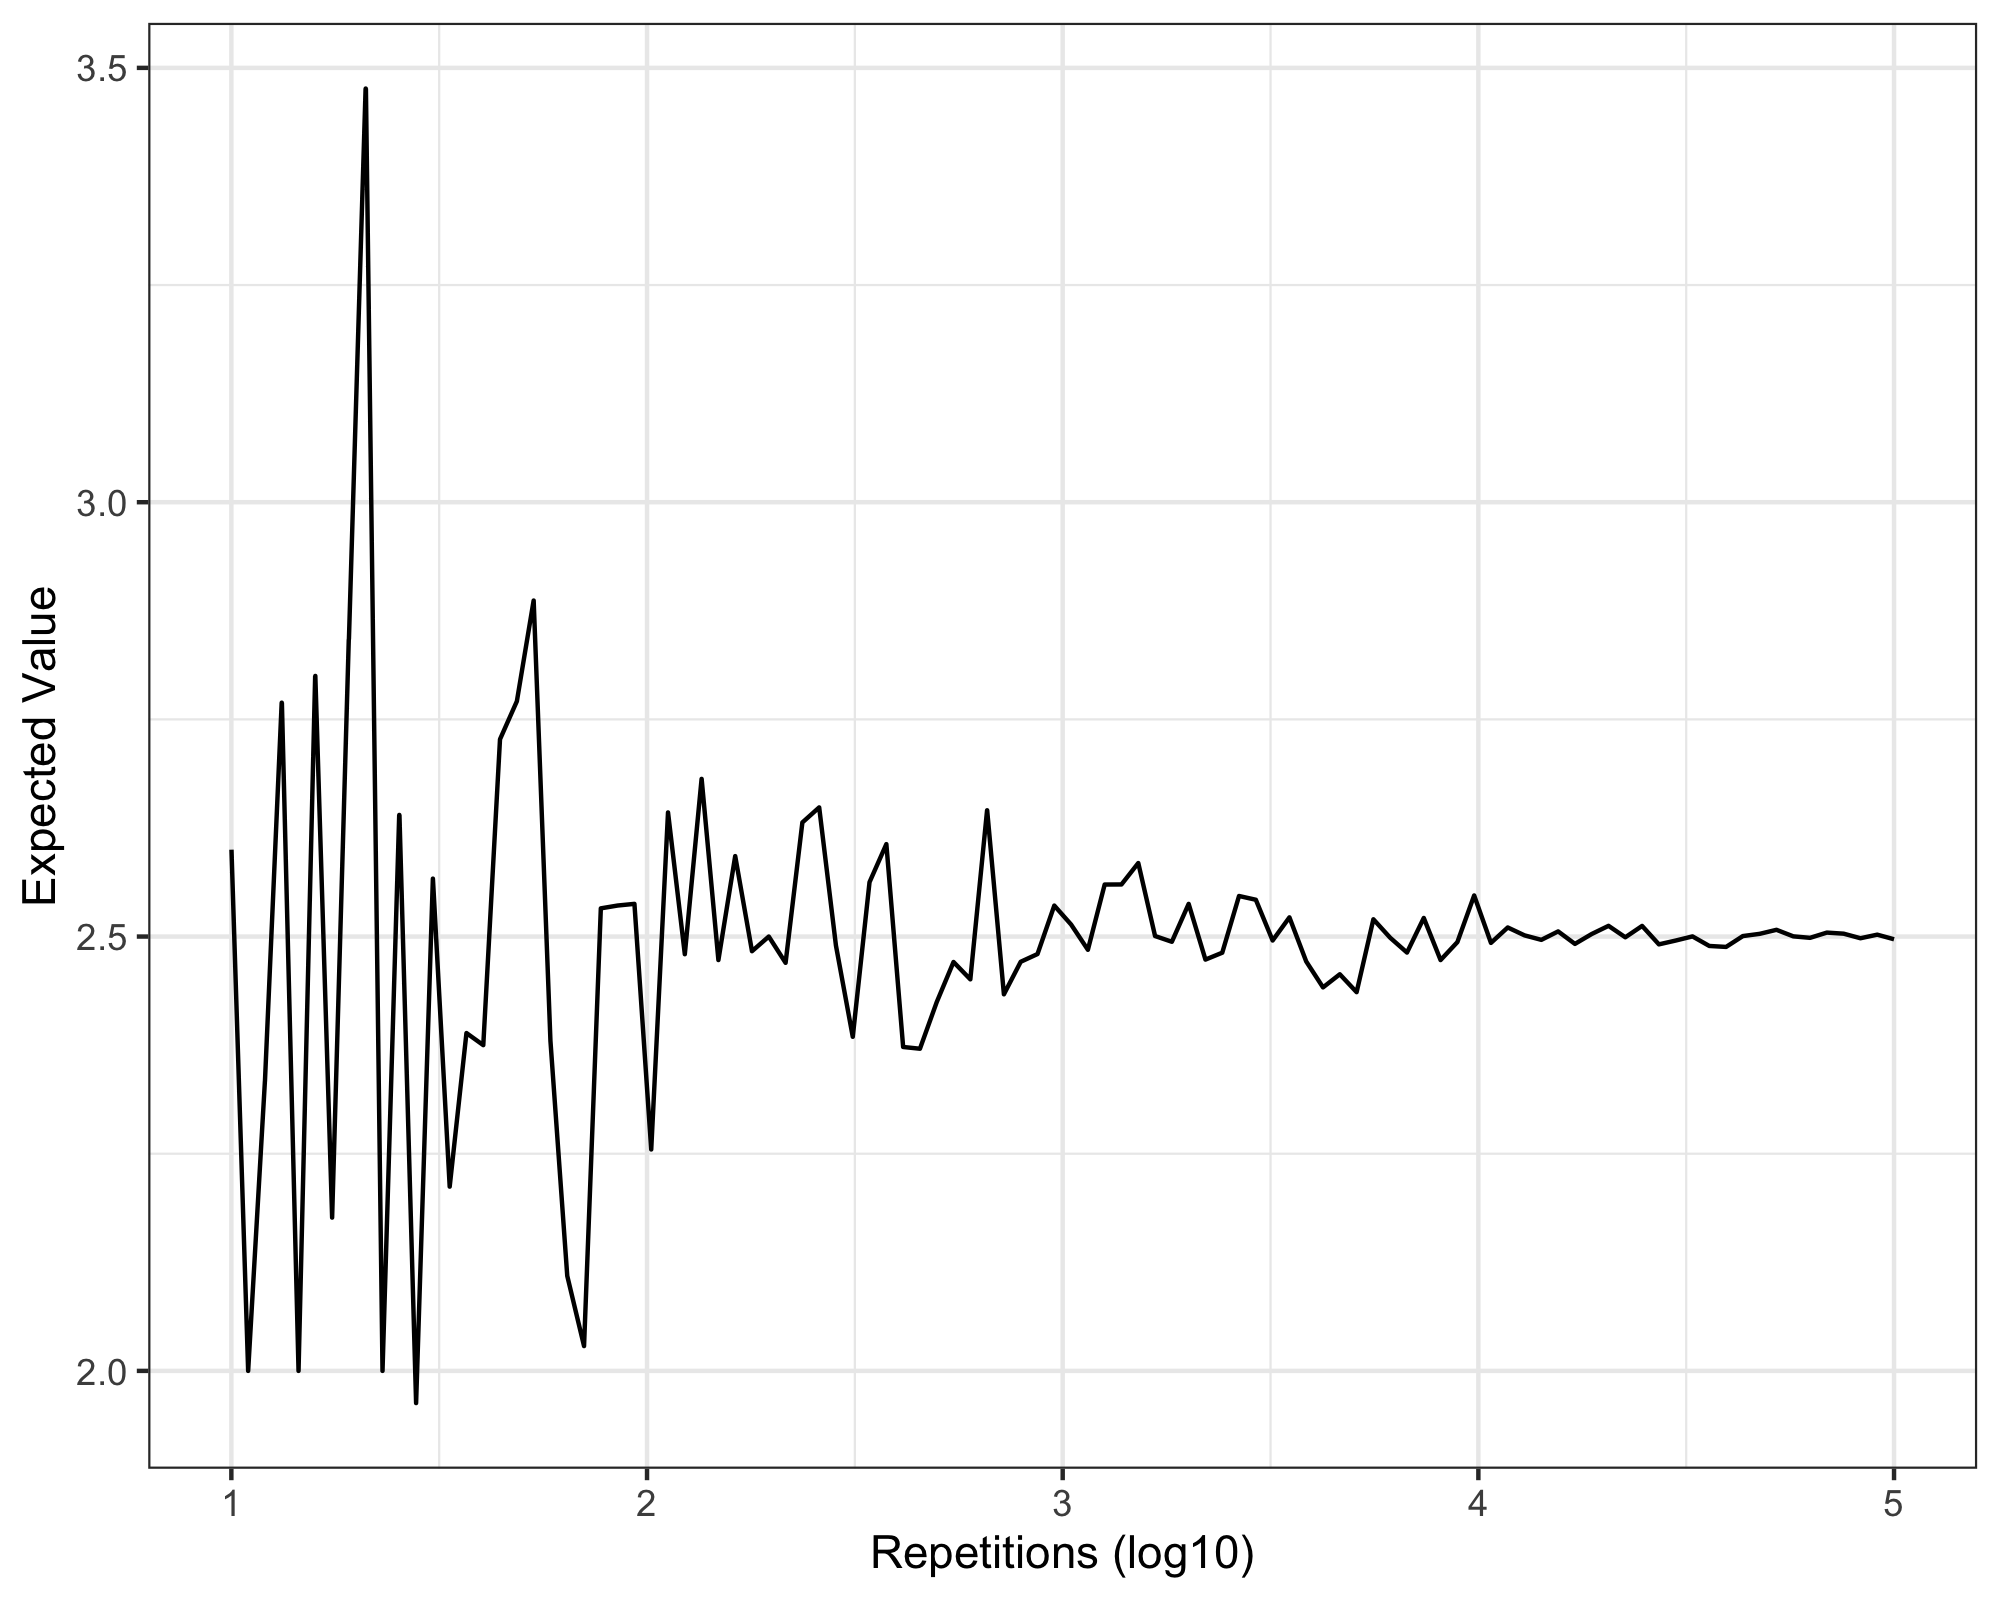
\includegraphics[scale=0.15]{img/plot_MC_18_249}
		\captionof{figure}{Stabilization of the expected value in the number of tries before opening the door in Exercise 18 page 249}
		\label{fig:plotrepMC}
	\end{center}
\end{figure}

	\subsection{Exercise 3 page 278}

For this exercise, the density function of the variable lifetime (in hours) of the ACME super light bulb is given. The calculated expected value $E(T) = 40$. The plot of the density function is generated and shown in Figure \ref{fig:dens}, which shows the highest area of the curve around the calculated expected value of 40.


\begin{figure}
	\begin{center}
		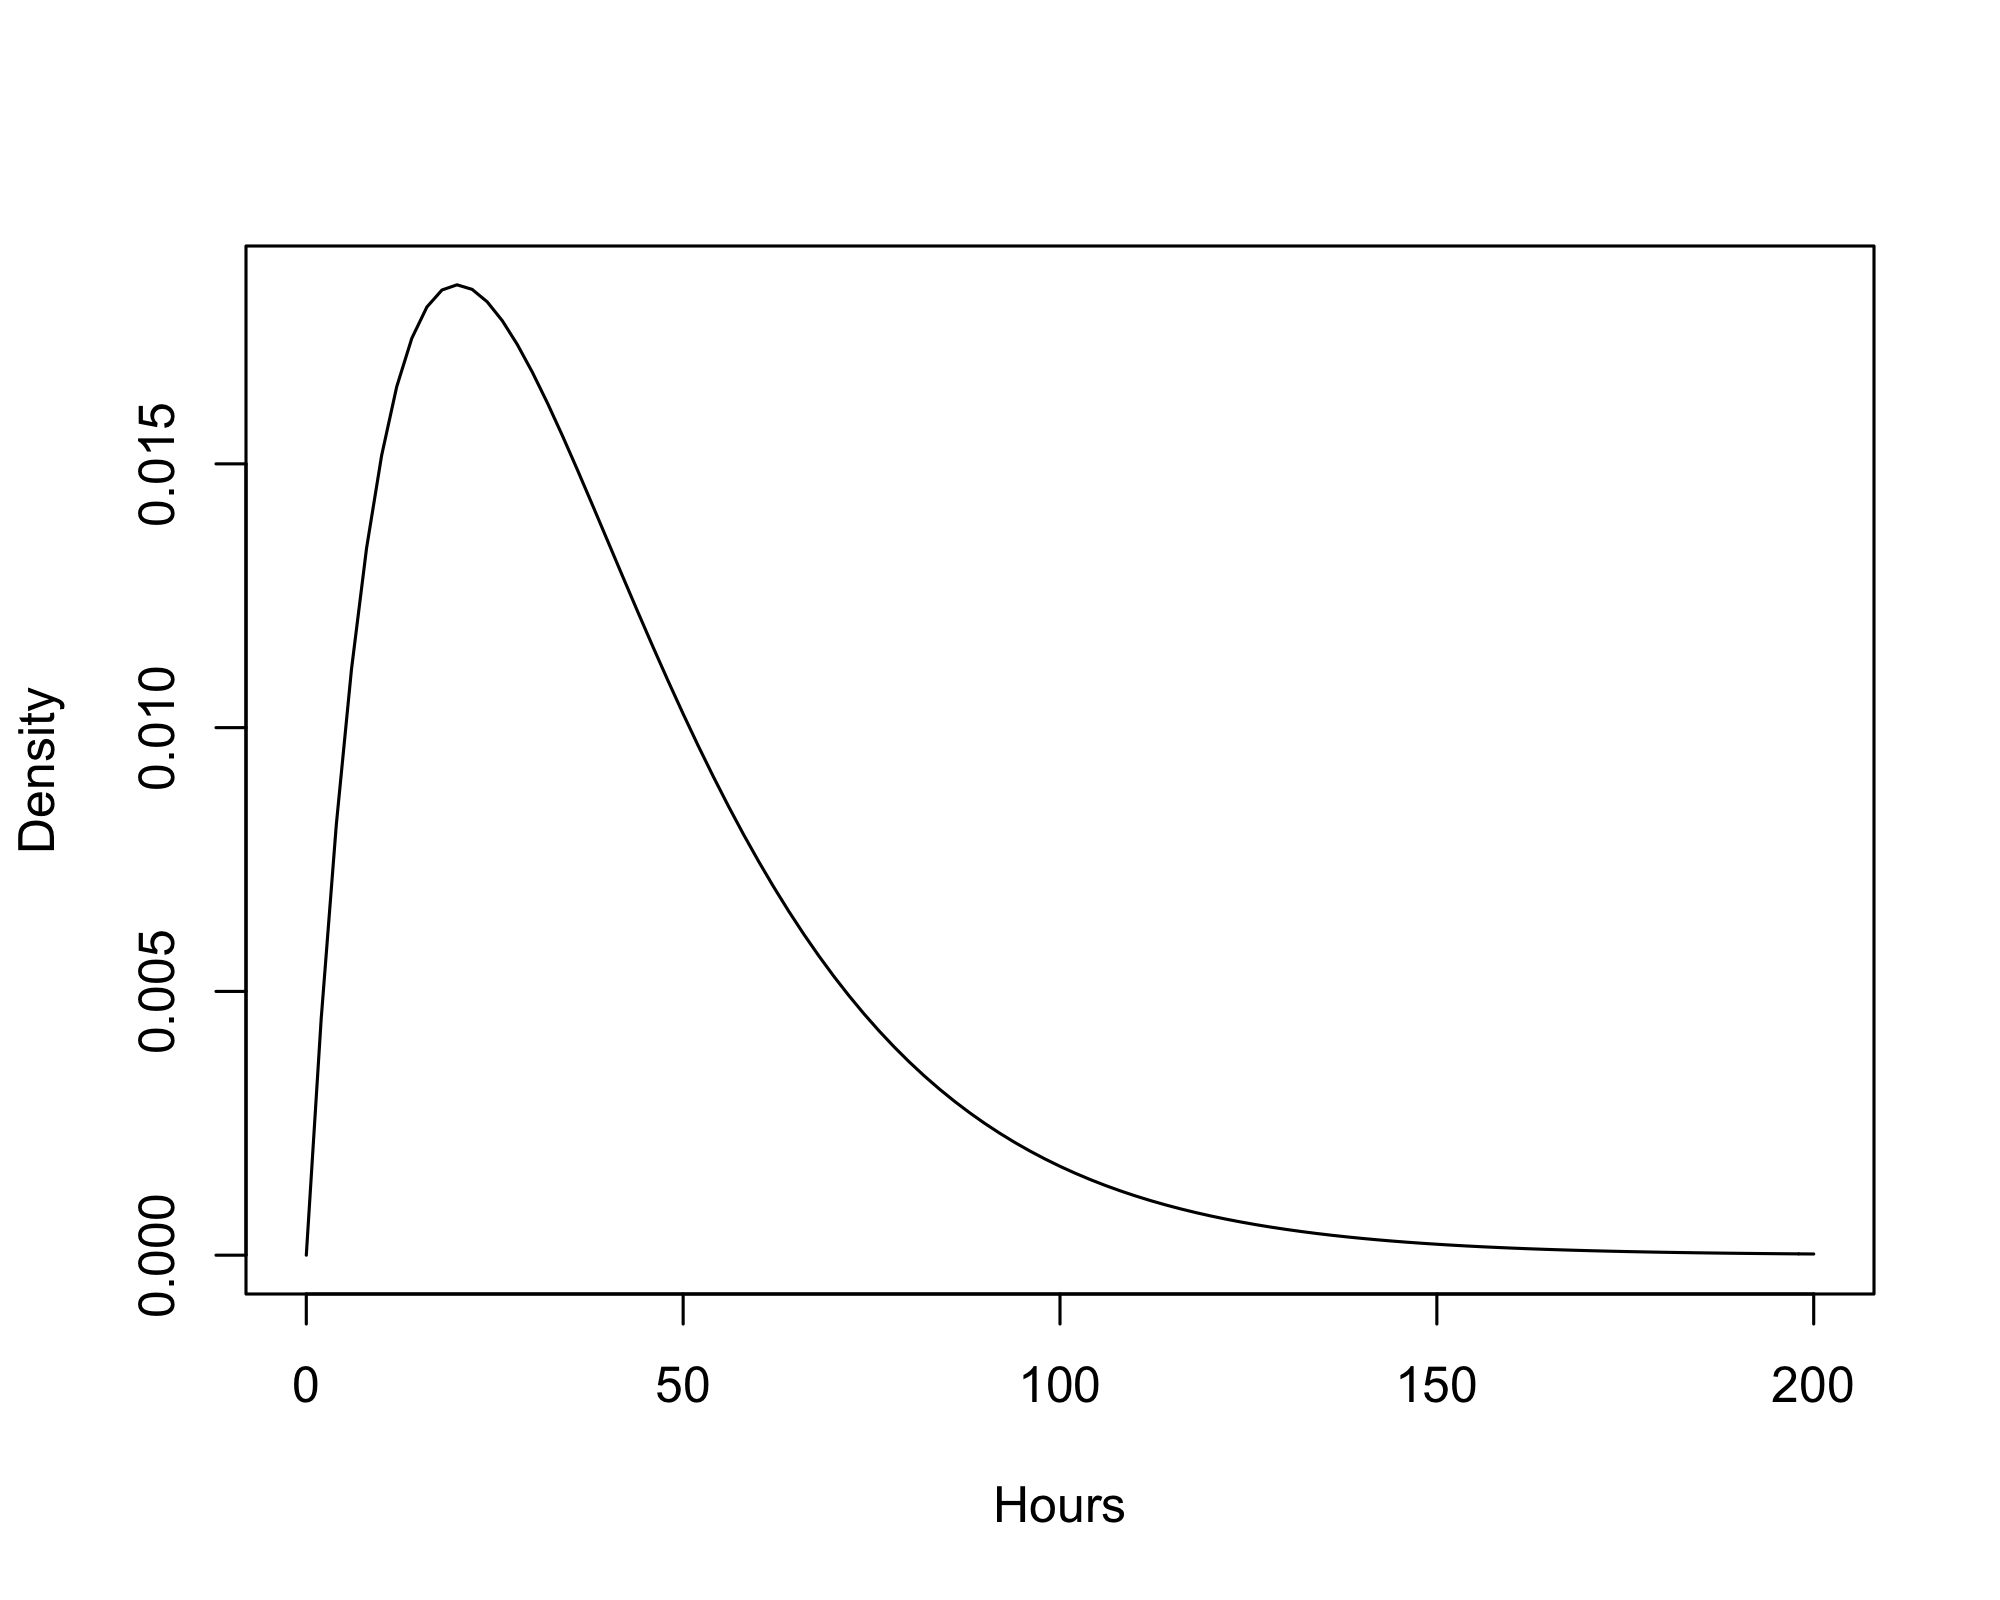
\includegraphics[scale=0.15]{img/dens_3_278}
		\captionof{figure}{Density curve of the lifetime of the light bulb in Exercise 3 page 278}
		\label{fig:dens}
	\end{center}
\end{figure}

\subsection{Exercise 12 page 280}

The variables $ X $ and $ Y $ are independent, and both are uniformly distributed on $\left[ 0,1\right]$.  The calculated expected value $E(X^{Y}) = \ln2$; this value correspond approximately to 0.6931. Simulations are shown in the histogram of Figure \ref{fig:hist12p280} and Figure \ref{fig:dotMC}, the latter shows how the expected value begin to stabilize as the number of repetition grows around the previously calculated value.


\begin{figure}
	\begin{center}
		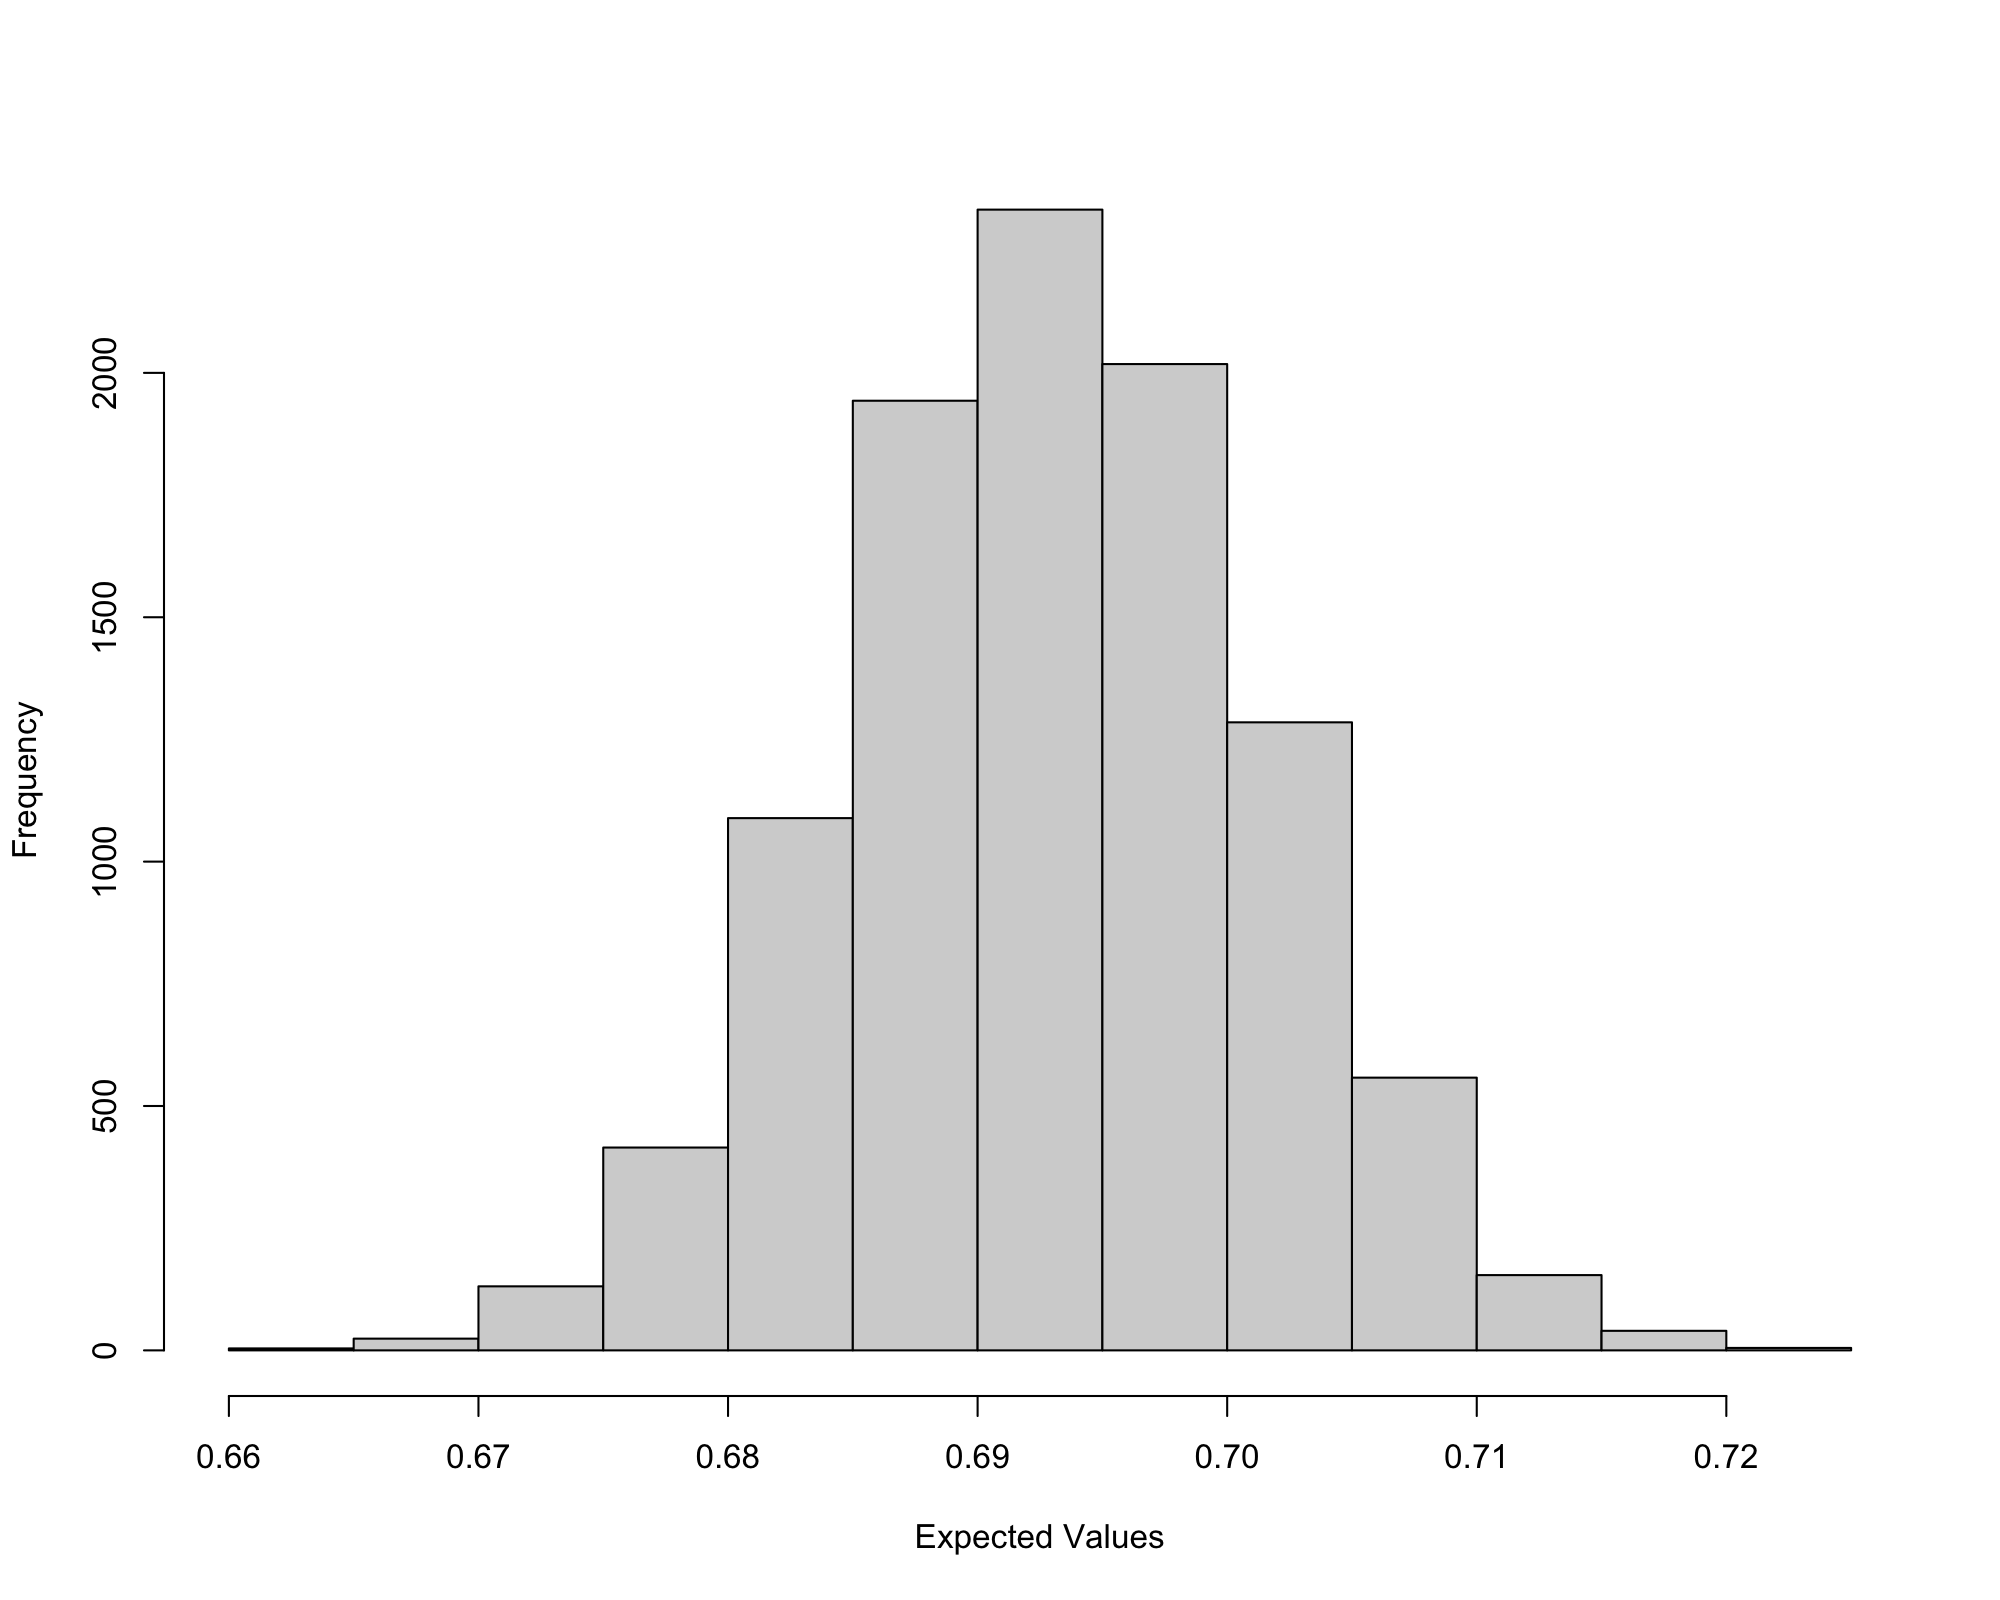
\includegraphics[scale=0.18]{img/hist12_280}
		\captionof{figure}{Histogram of the simulated expected values in Exercise 12 page 280}
		\label{fig:hist12p280}
	\end{center}
\end{figure}

\begin{figure}
	\begin{center}
		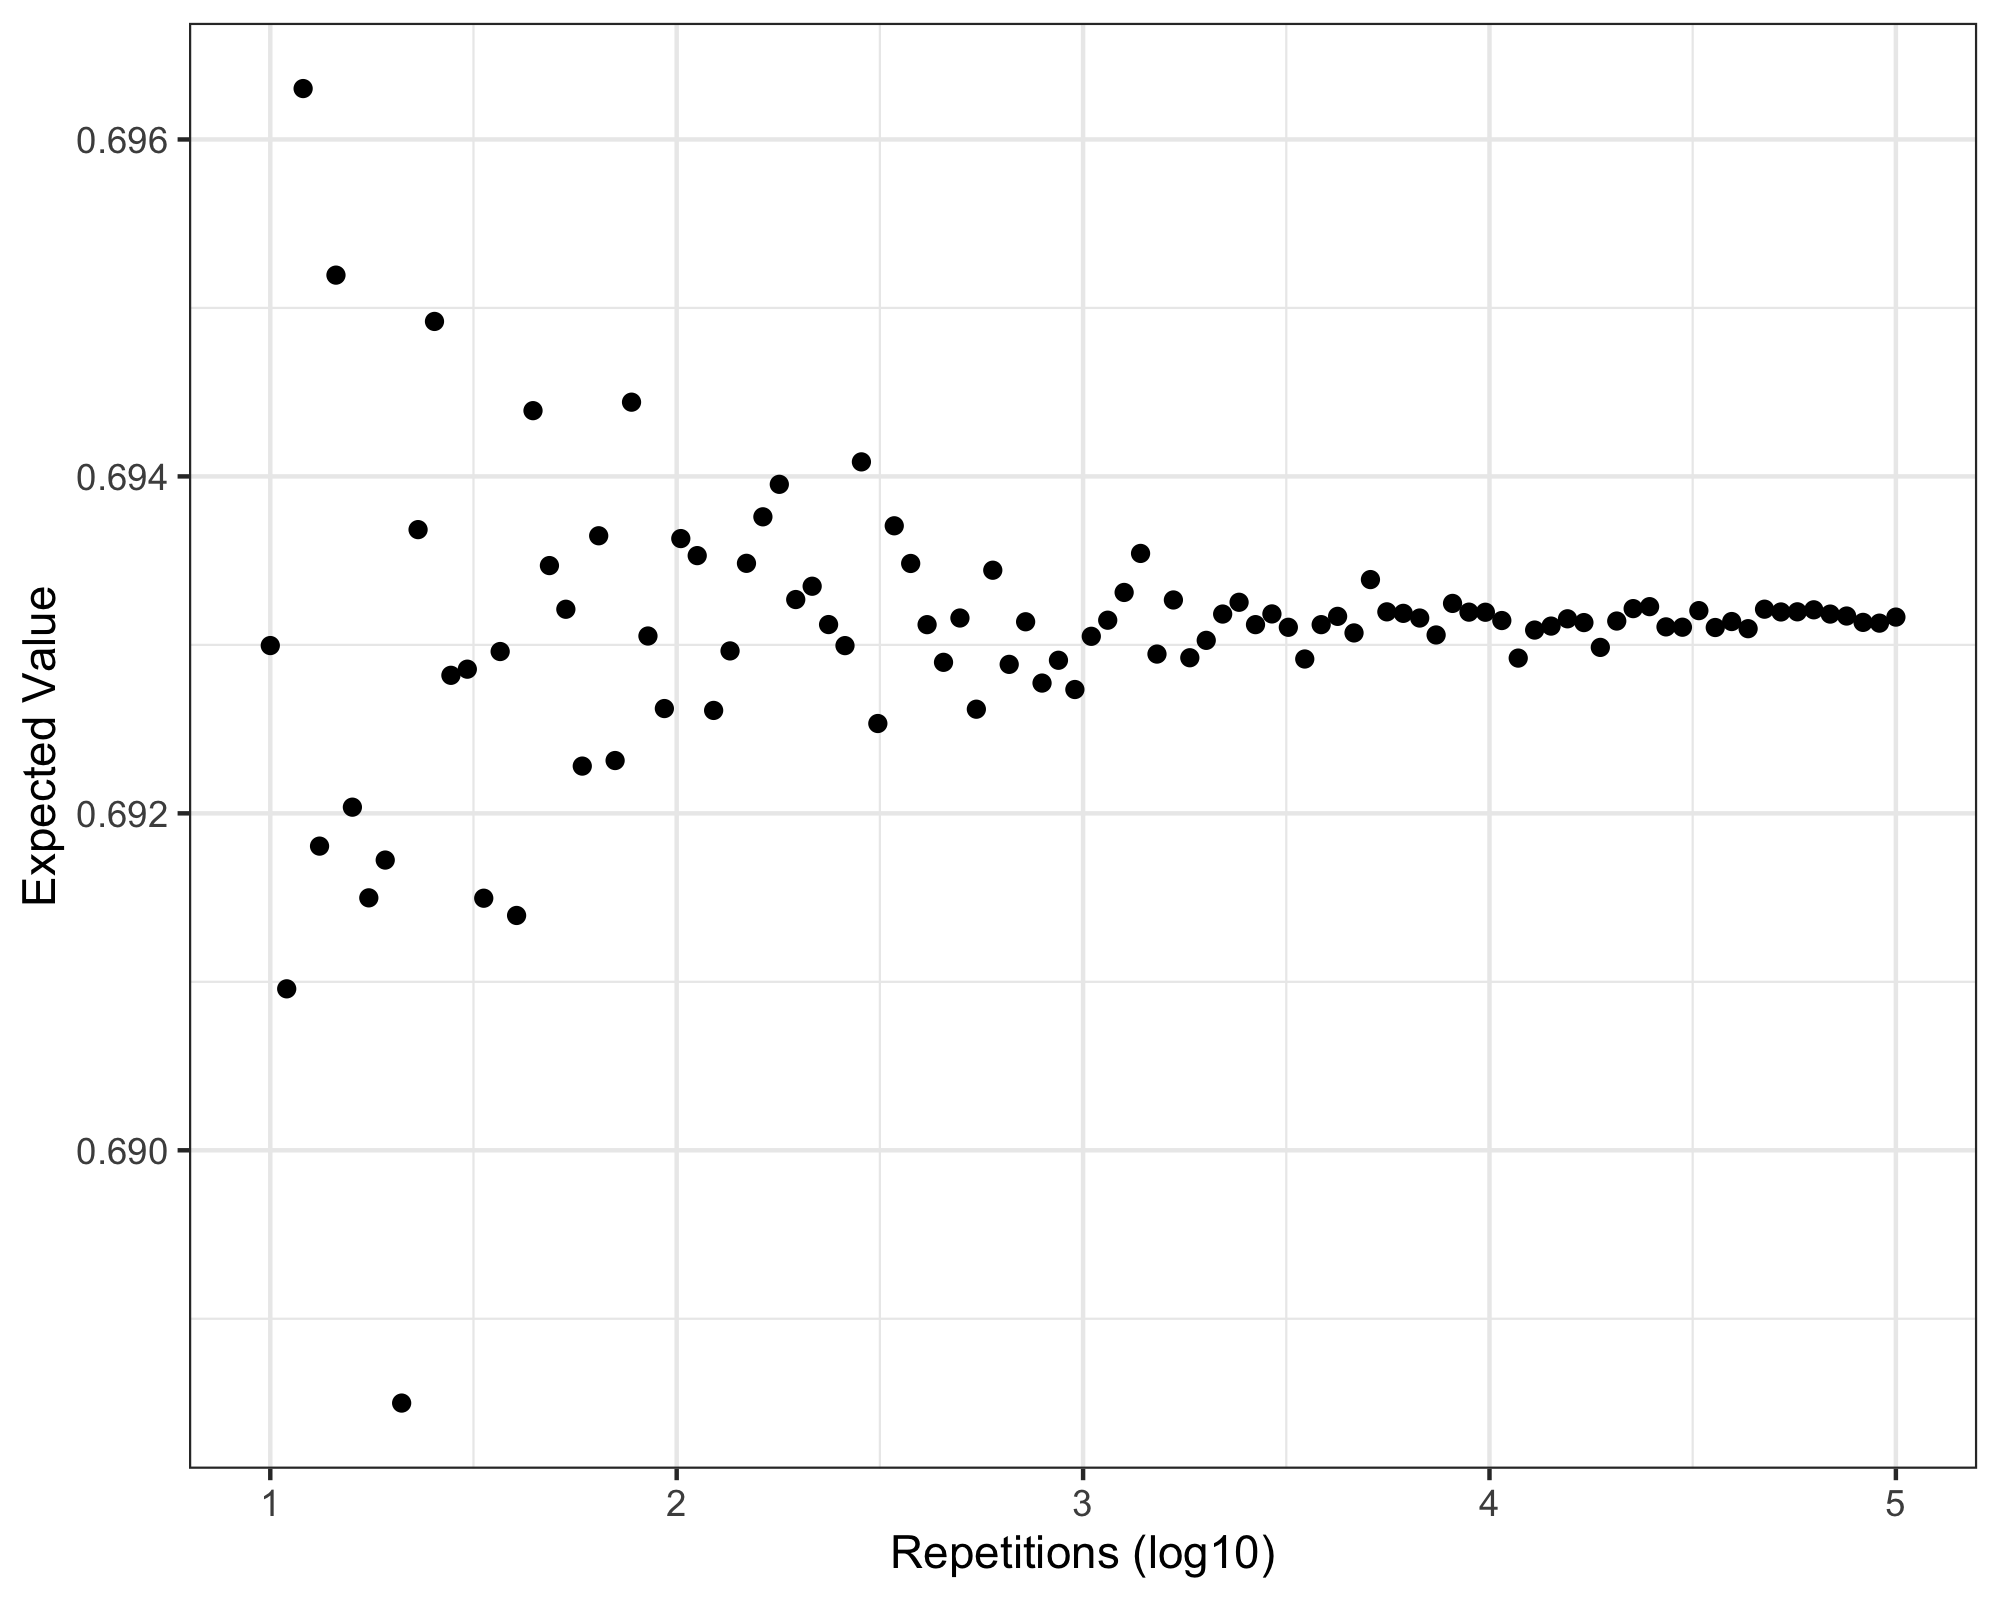
\includegraphics[scale=0.18]{img/plot_MClog2}
		\captionof{figure}{Stabilization of expected values in Exercise 12 page 280}
		\label{fig:dotMC}
	\end{center}
\end{figure}

			
\clearpage

	\bibliography{t10}
	\bibliographystyle{plainnat}

\end{document}